The Standard Model (\SM)~\cite{Peskin:257493} 
is a name given in 1970s to a theory describing the fundamental particles and their interactions. This quantum field theory describes the particles and their interactions as fields and has successfully incorporated three of the four fundamental forces in the universe. In \Sec{sec:SMcontent}, the particle content of the \SM\ is summarised, while \Sec{sec:SMlagr} describes  the \SM\ Lagrangian and its symmetries. In \Sec{sec:FCNC}, the flavour content of the \SM\ is highlighted. The successful theory of the \SM\ has some shortcomings which are discussed in \Sec{sec:BSM} and lead to searches for a more general theory. One of such a search is using effective field theory (EFT). In \Sec{sec:EFT} an EFT model focussing on flavour changing neutral currents (FCNC) involving a top quark is presented. Its current experimental constraints are given in \Sec{sec:ExpConstr}.

The physics search presented in this thesis relies on statistical tools and interpretations. In \Sec{sec:Stat}, the notion of a likelihood is presented as well as maximum likelihood fits. To set upper limits on a signal process the confidence levels method is used. The background modelling is checked using goodness-of-fit tests. Furthermore, the search will use multivariate analysis methods which are also explained.


\section{Elementary particles and forces}
\label{sec:SMcontent}
The interactions in nature can be described by four forces, the strong force, the electromagnetic (EM) force, the weak force and the gravitational force. These interactions happpen via particles with an integer spin known as bosons. The strong interaction is mediated by eight gluons \Pgluon, while the electromagnetic force is mediated by photons \Pphoton, and the weak force by \PZ and \PWpm bosons. In \tab{tab:forces}, the forces and their characteristics are shown. The gravitational force is the only force not included in the \SM\ and can be neglected for energies lower than the Planck scale (1.22 $10^{19}$ \GeV).
\begin{table}[htbp]
	\centering
	\caption{The four forces of nature and their characteristics.}
	\begin{tabular}{lcc}
		\toprule
		& Range & Mediator \\ 
		\midrule
		Strong force & $10^e{-15}$ \m & 8 gluons  \\ 
	
		Electromagnetic force & $\infty$ & photon  \\ 
		 
		Weak force & $10^{-18}$ \m & \PWpm, \PZ bosons \\ 
		
		Gravitational force & $\infty$ & unknown \\ 
		\bottomrule
	\end{tabular} 
	\label{tab:forces}
\end{table}

The fermions are the particles that make up the visible matter in the universe. They carry half integer spin and can be subdivided into leptons and quarks, where leptons don't interact strongly. Each fermion has a corresponding anti-fermion which has the same mass and is oppositely charged. The electron \Pelectron is the first elementary particle discovered~\cite{electrondiscovery} and belongs to the first generation of leptons together with electron neutrino \Pnue. The second generation is made up of the muon \Pmuon and the muon neutrino \Pnum, whereas the third generation consists of the tau \Ptau and the tau neutrino \Pnut. The neutrino's are neutral particles, while the other leptons have charge $\pm \qe$ where \qe represents the elementary charge of 1.602 $10^{-19}$ C. The masses of the charged leptons differ by four orders of magnitude between the first and third generations.In the \SM\ the neutrino's are assumed to be massless, while it is experimentally established that neutrino do have a tiny non-zero mass. In \tab{tab:leptongen}, the leptons and their properties in the \SM\ are summarised. 
\begin{table}[htbp]
	\centering
	\caption{The properties of the leptons in the three generations of the \SM~\cite{PDG}, where \qe represents the elementary  charge.}
	\begin{tabular}{lccc}
		\toprule
		Generation & Particle  & Mass  & Charge \\ 
		\midrule
		\multirow{2}{*}{First} & \Pelectron & 0.511 \MeV & -\qe  \\ 
		& \Pnue & $\approx$ 0 & 0\\
		
	\multirow{2}{*}{Second} & \Pmuon & 106 \MeV &-\qe  \\ 
	& \Pnum & $\approx$ 0 & 0\\
	
	\multirow{2}{*}{Third} & \Ptau & 1 777 \MeV & -\qe  \\ 
	& \Pnut & $\approx$ 0 & 0 \\
	
		
		\bottomrule
	\end{tabular} 
	\label{tab:leptongen}
\end{table}

The quarks can also be divided into three generations. Unlike the leptons, they carry colour charge and can interact via the strong interaction. The top quark, discovered in 1995 at the Tevatron~\cite{observationtopD0,observationtopCDF} is the heaviest \SM\ particle with a mass close to $173.1\pm0.6$ \GeV\footnote{In this thesis all masses and energies are expressed in natural units, where the speed of light and $\hbar$ are taken to be equal to one.}~\cite{PDG}. The quarks and their properties are summarized in \tab{tab:quarkgen}. In nature, only colour neutral objects can exist. This has as consequence that quarks are bound through gluons into mesons (quark+anti-quark) and baryons (three quarks). These mesons and baryons are mostly short-lived and unstable particle that rapidly decay through \PWpm\ and \PZ\ bosons, associated with a fermion. The only known stable baryon is the proton, made up of two up quarks and one down quark.  
\begin{table}[htbp]
	\centering
	\caption{The properties of the quarks in the three generations of the \SM~\cite{PDG}, where \qe represents the elementary  charge.}
	\begin{tabular}{lccc}
		\toprule
		Generation & Particle  & Mass  & Charge \\ 
		\midrule
		\multirow{2}{*}{First} & up \Pup &$2.2_{-0.4}^{+0.6}$ \MeV& $\textfrac{2}{3}$ \qe  \\ 
		& down \Pdown & $4.7^{+0.5}_{-0.4}$ \MeV & $\textfrac{-1}{3}$ \qe\\
		
		\multirow{2}{*}{Second} & charm \Pcharm & 1.28 $\pm$ 0.03 \GeV &$\textfrac{2}{3}$ \qe  \\ 
		& strange \Pstrange & $96^{+8}_{-4}$ \MeV & $\textfrac{-1}{3}$ \qe\\
		
		\multirow{2}{*}{Third} & top \Ptop & 173.1 $\pm$ 0.6 \GeV &$\textfrac{2}{3}$ \qe  \\ 
		&bottom \Pbottom & $4.18^{+0.04}_{-0.03}$ \GeV & $\textfrac{-1}{3}$ \qe \\
		
		
		\bottomrule
	\end{tabular} 
	\label{tab:quarkgen}
\end{table}

The scalar boson, commonly known as the Higgs boson, is the last piece of the \SM\ and is discovered in 2012~\cite{Chatrchyan:2012xdj,Aad:2012tfa}. It is responsible for the masses of the \PWpm and \PZ boson, and that of the fermions.


\section{Standard Model Lagrangian}
\label{sec:SMlagr}
The \SM\ is a quantum field theory and thus describes the dynamics and kinematics of particles and forces by a Lagrangian \Lagr. The theory is based on the \SSU\ gauge symmetry, where \SU\ describes the electroweak interaction and \Sthree\ the strong coupling. The indices refer to colour C, the left chiral nature of the \Stwo\ coupling L, and the weak hypercharge Y. Its Lagrangian is constructed such that contains symmetries representing physics conservation laws such as conservation of energy, momentum and angular momentum. By imposing gauge invariance {\todo{should I explain gauge invariance or is a reference enough?}} the symmetries under local group transformations are sustained. 



The \Uone\ group has one generator Y with an associated gauge field \Bfield. The three gauge fields \Wfieldone, \Wfieldtwo, and \Wfieldthree, are associated to \Stwo with three generators that can can  be written as half of the Pauli matrices: 
\begin{equation}
T_1 =  \frac{1}{2}
\begin{pmatrix}
0  &  1      \\
1  & 0      
\end{pmatrix}, \;
T_2= \frac{1}{2}
\begin{pmatrix}
0  &  -i     \\
i  &  0      
\end{pmatrix},\;\mathrm{ and } \;
 T_3= \frac{1}{2}
 \begin{pmatrix}
 1  &  0     \\
 0  &  -1 
 \end{pmatrix}.
\end{equation}
The generators $T^a$ satisfy the Lie algebra: 
\begin{equation}
 \left[T^a,T^b\right] = i \epsilon^{abc} T_c \; \mathrm{ and } \left[T^a, Y\right] = 0, 
\end{equation}
where $\epsilon^{abc}$ is an antisymmetric tensor. The gauge fields of \Stwo\ only couple to left-handed fermions as required by the observed parity violating nature of the weak force. The \Sthree\ group represents quantum chromodynamics (QCD). It  has eight generators corresponding to eight gluon fields \Gfields. Unlike \SU, \Sthree\ is not chiral. 

Under \Sthree\, quarks are colour triplets while leptons are colour singlets. This implies that the quarks carry a colour index ranging between one and three, whereas leptons do not take part in strong interactions. Based on the chirality, the quarks and leptons are organized in doublets or singlets. Each generation $i$ of fermions consists of left-handed doublets and right-handed singlets: 
\begin{equation}
\mathrm{l}_{\mathrm{L}} =  
\begin{pmatrix}
\Pelectron_{\mathrm{L}}       \\
\Pneutrino_{\mathrm{L}}     
\end{pmatrix}, \; \Pelectron_{\mathrm{R}}, \; \mathrm{q}_{\mathrm{L}} = 
\begin{pmatrix}
\Pup_{\mathrm{L}}       \\
\Pdown_{\mathrm{L}}     
\end{pmatrix}, \; \Pup_{\mathrm{R}}, \; \mathrm{and} \; \Pdown_{\mathrm{R}}
\end{equation}

The \SM\ Lagrangian can be decomposed as a sum of four terms
\begin{equation}
\lagr_{\mathrm{SM}} = \lagr_{\mathrm{gauge}} + \lagr_{\mathrm{f}} + \lagr_{\mathrm{Yuk}} + \lagr_{\phi}, 
\end{equation}
that are related to the gauge, fermion, Yukawa and scalar sectors. The gauge Lagrangian regroups the gauge fields of all three symmetry groups, and the fermionic part consists of kinetic energy terms for quarks and leptons. The interaction between fermions and the scalar doublet $\phi$ gives rise to fermion masses and is described by the Yukawa Lagrangian. The scalar part of the Lagrangian is composed of a kinematic and potential component related to the scalar boson. 
%\begin{equation}
% \lagr_{\mathrm{gauge}} = -\frac{-1}{4} \Gtensord \Gtensoru -\frac{-1}{4} \Wtensord \Wtensoru - -\frac{-1}{4} \Btensord \Btensoru, 
%\end{equation}
%where the tensors are
%\begin{align}
%\Gtensord &= \partial_{\mu}\mathrm{G}_{\nu}^i - \partial_{\nu}\mathrm{G}_{\mu}^i - g_{\mathrm{s}} f_{ijk} \mathrm{G}_{\mu}^j \mathrm{G}_{\nu}^k, \; \mathrm{ with }\; i,j,k = 1,...,8 \\
%\Wtensord &= \partial_{\mu}\mathrm{W}_{\nu}^i - \partial_{\nu}\mathrm{W}_{\mu}^i - g_{\mathrm{s}} \epsilon_{ijk} \mathrm{W}_{\mu}^j \mathrm{G}_{\nu}^k, \; \mathrm{ with }\; i,j,k = 1,...,8 \\
%\end{align}

For the electroweak theory, two coupling constants are introduced, namely $g'$ for \Uone\ and $g$ for \Stwo. The physically observable gauge bosons of this theory are the photon field \photonfield, the \PZ\ boson field \Zfield, and the \PW\ field \Wfield. These are a superposition of the four gauge fields of \SU: 
\begin{equation}
\photonfield = \sW \Wfieldone + \cW \Bfield, \; \Zfield = \cW \Wfieldthree - \sW \Bfield, \; \mathrm{ and } \; \Wfield = \sqrt{\frac{1}{2}}\left(\Wfieldone\mp \Wfieldtwo\right), 
\end{equation}
where $\theta_{\mathrm{W}}$ represents the weak mixing angle defined as $\mathrm{tan} \theta_{\mathrm{W}} = \frac{g'}{g}$.

The coupling constant representing the strength of the QCD interactions is denoted as $g_{\mathrm{s}}$. In QCD their is asymptotic freedom whereby the strong coupling constant becomes weaker as the energy with which the interaction between strongly interacting particles is probed increases, and stronger as the distance between the particles increases. A consequence of this is known as colour confinement. The quarks and gluons can not exist on their own and are not observed individually. They are bound in colour neutral states called hadrons, this process is known as hadronisation. 
\subsection*{Electroweak symmetry breaking}
In $\lagr_{\mathrm{gauge}}$ and $\lagr_{\mathrm{f}}$ are no mass terms for fermions present because only singlets under \SSU\ can acquire a mass with an interaction of the type $m^2\phi^{\dagger}\phi$ without breaking the gauge invariance. In order to accommodate mass terms for fermions and gauge fields, electroweak symmetry breaking, leading to $\lagr_{\phi}$ is introduced. 

The scalar doublet is introduced in the \SM\ as 
\begin{equation}
\phi = \frac{1}{\sqrt{2}}
\begin{pmatrix}
\varphi_1 + i \varphi_2    \\
\varphi_3 + i \varphi_4    
\end{pmatrix}.
\end{equation}
Its field potential is of the form \todo{check if I need to add constants here}
\begin{equation}
V(\phi) = \mu^2 \phi^{\dagger}\phi + \lambda(\phi^{\dagger}\phi)^2, 
\end{equation}
with $\mu^{2} <0$ and $\lambda$ a positive integer. This choice of parameters gives the potential a "Mexican hat" shape. I has an infinite set of minima (ground states) and by expanding the field around an arbitrary choice of ground state, the electroweak symmetry is broken (\cancel{EW}): 
\begin{equation}
\phi = 
\begin{pmatrix}
0    \\
\frac{v}{\sqrt{2}}    
\end{pmatrix}
+ \hat{\phi}, 
\end{equation}
where $v$ is the vacuum expectation value (vev), measured to be around 245 \GeV\ and corresponds to $\sqrt{\frac{-\mu}{\lambda}}$. The scalar doublet's four degrees of freedom is reduced to three degrees of freedom that couple to the gauge fields and mix with the \PWp, \PWm and \PZ bosons. The remaining fourth degree of freedom has given rise ta physically observable particle , called the Brout-Englert-Higgs (BEH) boson.
This spontaneous symmetry breaking leaves the gauge invariance intact and gives masses to the \PWpm and \PZ bosons as:
\begin{equation}
m_{\PW} = \frac{1}{2}v|g| \quad \mathrm{and} \quad m_{\PZ} = \frac{1}{2}v \sqrt{g'^2 + g^2}.
\end{equation}
The Brout-Englert-Higgs field couples universally fermions with a strength proportional to their masses, and to gauge bosons with a strength proportional to the square of their masses. 


\section{Flavour changing currents in the \SM}
\label{sec:FCNC}
%In the electroweak theory, the \PW boson is responsible for flavour changing charged currents, and the \PZ boson for 
%lading W -> smamak veranderen -> niet voor Z , integendeel verboden op tree level onderdrukt op higher order
Flavour changing charged currents are introduced in 1963 by Nicola Cabibbo~\cite{PhysRevLett.10.531}. Via interaction with a \PW boson the flavour of the quarks is changed. At the time of the postulation, only up, down and strange quarks were known and the charged weak current was described as a coupling between the up quark and $\Pdown_{\mathrm{weak}}$, where $\Pdown_{\mathrm{weak}}$ is a linear combination of the down and strange quarks, $\Pdown_{\mathrm{weak}}= \mathrm{cos }\theta_{\mathrm{c}} \Pdown + \mathrm{sin }\theta_{\mathrm{c}} \Pstrange$. This linear combination is a direct consequence of the chosen rotation
\begin{equation}
\begin{pmatrix}
\Pdown_{\mathrm{weak}} \\
\Pstrange_{\mathrm{weak}} 
\end{pmatrix}
 = 
 \begin{pmatrix}
 \mathrm{cos }\theta_{\mathrm{c}} &  \mathrm{sin }\theta_{\mathrm{c}} \\
 - \mathrm{sin }\theta_{\mathrm{c}} &  \mathrm{cos }\theta_{\mathrm{c}}
 \end{pmatrix}
 \begin{pmatrix}
 \Pdown \\
 \Pstrange 
 \end{pmatrix} = \mathcal{R} 
 \begin{pmatrix}
 \Pdown \\
 \Pstrange 
 \end{pmatrix}, 
\end{equation}
where the rotation angle $\theta_{\mathrm{c}}$ is known as the Cabibbo angle. This provides a definition for the charged weak current between \Pup and \Pdown quarks, 
\begin{equation}
J_{\mu} = \bar{\Pmu} \gamma_{\mu}\left(1+\gamma_5\right)\Pdown_{\mathrm{weak}}. 
\end{equation} 
A consequence of Cabibbo's approach is that the $\Pstrange_{\mathrm{weak}}$ is left uncoupled, leading to Glashow, Iliopoulos and Maiani (GIM)~\cite{PhysRevD.2.1285,BJORKEN1964255,Maiani:2013fpa} to require the existence of a fourth quark with charge $\textfrac{2}{3}$. This quark, known as the charm quark, couples to $\Pstrange_{\mathrm{weak}}$ and a new definition of the charged weak current is modified to 
\begin{equation}
J_{\mu} = \begin{pmatrix}
u & c
\end{pmatrix}  \gamma_{\mu}\left(1+\gamma_5\right)\mathcal{R}  \begin{pmatrix}
d \\ s
\end{pmatrix}
= \bar{U} \gamma_{\mu}\left(1+\gamma_5\right)\mathcal{R}D. 
\end{equation} 

The neutral weak current is defined as 
\begin{equation}
J_{3} = \bar{U} \gamma_{\mu}\left(1+\gamma_5\right)\left[\mathcal{R}, \mathcal{R}^{\dagger}\right]D, 
\end{equation} 
and is diagonal in flavour space. This has as consequence that no flavour changing neutral currents occur at tree-level Feynmann diagrams\footnote{Feynmann diagrams are physical representation of interaction between particles. They are based on Feynmann rules~\cite{Peskin:257493}.} \todo{should I explain feynmann diagrams?}.


Kobayashi and Maskawa generalised the Cabibbo rotation matrix to accommodate for a third generation of quarks. The result is a $3\times 3$ unitary matrix known as the CKM matrix, responsible for the mixing of weak interaction states of down-type quarks: 
\begin{equation}
\begin{pmatrix}
\Pdown_{\mathrm{weak}} \\
\Pstrange_{\mathrm{weak}} \\
\Pbottom_{\mathrm{weak}}
\end{pmatrix}
= 
\begin{pmatrix}
V_{\Pup\Pdown} & V_{\Pup\Pstrange} & V_{\Pup\Pbottom} \\
V_{\Pcharm\Pdown} & V_{\Pcharm\Pstrange} & V_{\Pcharm\Pbottom} \\
V_{\Ptop\Pdown} & V_{\Ptop\Pstrange} & V_{\Ptop\Pbottom}
\end{pmatrix}
\begin{pmatrix}
\Pdown \\
\Pstrange \\
\Pbottom
\end{pmatrix} = \mathcal{V}_{\mathrm{CKM}} \begin{pmatrix}
\Pdown \\
\Pstrange \\
\Pbottom
\end{pmatrix}.
\end{equation}
The unitarity of the matrix ($\mathcal{V}_{\mathrm{CKM}}^{\dagger}\mathcal{V}_{\mathrm{CKM}} = \mathbb{1}$). A general $3\times 3$ unitary matrix depends on three real angles and six phases. For the CKM matrix, the freedom to redefine the phases of the quark eigenstates can remove fives of the phases, leaving a single physical phase known as the Kobayashi-Maskawa phase. This phase is responsible for the charge parity violation in the \SM~\cite{CKM}. 
% see wolfenstein parametrisation http://pdg.lbl.gov/2017/reviews/rpp2016-rev-cp-violation.pdf 13,53
Each element $V_{\mathrm{ij}}$ of $ \mathcal{V}_{\mathrm{CKM}}$ represents the transition probability of a quark i going to a quark j, and is experimentally determined to be~\cite{PDG}
\begin{equation}
\mathcal{V}_{\mathrm{CKM}} =
\begin{pmatrix}
0.97425 \pm 0.00022  & 0.2253 \pm 0.0008      & (4.13 \pm 0.49) 10^{-3} \\
0.225 \pm 0.008      & 0.986 \pm 0.016        & (41.1 \pm 1.3) 10^{-3} \\
(8.4\pm 0.6) 10^{-3} & (40.0 \pm 2.7) 10^{-3} & 1.021 \pm 0.032
\end{pmatrix}.
\label{eq:CKM}
\end{equation}

From  \eq{eq:CKM} follows that top quarks predominantly decay via charged weak currents to bottom quarks, with a probability consistently with unity. In the \SM, FCNC can only occur via higher loop Feynmann diagrams which are highly suppressed. The expected transition probabilities for a top quark decaying via a FCNC interaction in the \SM\ are given in \tab{tab:FCNCBR}, where it is clear that the FCNC sector of the \SM\ is still beyond the reach of the sensitivity of current experiments. 
\begin{table}[htbp]
	\centering
	\caption{The predicted branching ratios \BR\ for FCNC interactions involving the top quark in the \SM~\cite{AguilarSaavedra:2004wm}}
	\begin{tabular}{lclc}
		\toprule
	    Process	& \BR\ in the \SM  &  Process	& \BR\ in the \SM \\ 
		\midrule
		$ \Ptop \rightarrow \Pup \PZ $         & $8 \; 10^{-17}$  &	$ \Ptop \rightarrow \Pcharm \PZ $      & $1 \; 10^{-14}$   \\
		$ \Ptop \rightarrow \Pup \Pphoton $    & $4 \; 10^{-16}$  & $ \Ptop \rightarrow \Pcharm \Pphoton $ & $5 \; 10^{-14}$   \\
		$ \Ptop \rightarrow \Pup \Pgluon $     & $4 \; 10^{-14}$  & $ \Ptop \rightarrow \Pcharm \Pgluon $  & $5 \; 10^{-12}$  \\
		$ \Ptop \rightarrow \Pup \PHiggs $     & $2 \; 10^{-17}$  & $ \Ptop \rightarrow \Pcharm \PHiggs $  & $3 \; 10^{-15}$ \\
		\bottomrule
	\end{tabular} 
	\label{tab:FCNCBR}
\end{table}



\section{Motivations for new physics}
\label{sec:BSM}
\todo{Reread and elaborate}
Many high energy experiments confirm the success of the \SM. In particular the scalar boson, the cornerstone of the \SM, has consecrated the theory. Unfortunately there are also strong indications that the \SM\ ought to be a lower energy expression of a more global theory. The existence of physics beyond the \SM (BSM)~\cite{BSMWiley} is strongly motivated. These motivations are based on direct evidence from observation such as the existence of neutrino masses, the existence of dark matter and dark energy, or the matter-antimatter asymmetry, and also from theoretical problems such as the hierarchy problem, the coupling unification or the large numbers of free parameters in the \SM. 


In the \SM, the neutrino is assumed to be massless, whilst experiments with solar, atmospheric, reactor and accelerator neutrinos have established that neutrinos can oscillate and change flavour during flight~\cite{Fukuda:1998mi,PhysRevLett.108.131801}. These oscillations are only possible when neutrino's have masses. The flavour neutrinos (\Pnue, \Pnum, \Pnut) are then linear expressions of the fields of at least three mass eigenstate neutrinos \Pnu$_1$, \Pnu$_2$, and \Pnu$_3$. 

The ordinary or baryonic matter described by the \SM\ describes only 5\% of the mass (energy) content of the universe. Astrophysical evidence indicated that dark matter is contributing to approximately 27\%, and dark energy to 68\% of the content of the universe. From the measurements of the temperature and polarizations anisotropies of the cosmic microwave background by the Planck experiment~\cite{Ade:2015xua}, the density of cold non baryonic matter is determined. Cold dark matter is assumed to be only sensitive to the weak and gravitational force, leading to only one possible \SM\ candidate: the neutrino. However, these are too light to account for the vast amount of dark matter and other models are needed. Dark energy is assumed to be responsible for the acceleration in the expansion of the universe~\cite{Peebles:2002gy}. 
%https://en.wikipedia.org/wiki/Accelerating_expansion_of_the_universe#Evidence_for_acceleration

At the big bang matter and antimatter is assumed to be produced in equal quantities. However, it  is clear that we are surrounded by matter. So where did all the antimatter go? In 1967, Sakharov identified three mechanisms that are necessary to obtain a global matter antimatter asymmetry~\cite{Sakharov}. These mechanisms are baryon and lepton number violation, at a given moment in time there was a thermal imbalance for the interactions in the universe, and there is charge C and charge parity CP violation\footnote{The rate of a process $i\rightarrow f$ can be different from the CP-conjugate process: $\tilde i \rightarrow \tilde f$. The \SM\ includes sources of CP-violation through the residual phase of the CKM matrix. However, these could not account for the magnitude of the asymmetry observed.}.
% infor CP viol http://pdg.lbl.gov/2017/reviews/rpp2016-rev-cp-violation.pdf
% CP violation can occur in a filed theory when the lagrangian density involves more complex parameters than what can be removed by field redefinitions
The large numbers of free parameters in the \SM\ are taken as nine fermion masses, three CKM mixing angles and one CP violating phase, one EM coupling constant $g'$, one weak coupling constant $g$, one strong coupling constant $g_{\mathrm{s}}$, one QCD vacuum angle, one vacuum expectation value, and one mass of the scalar boson. This large number of free parameters lead to the expectation of a more elegant, general theory beyond the \SM. 

The hierarchy problem~\cite{Burdman:2007ck} is related to the huge difference in energy between the weak scale and the Planck scale. The vev of the Brout-Englert-Higgs field determines the weak scale that is approximately 246 \GeV.  The radiative corrections to the scalar boson squared mass $m_{\PH}^2$, coming from its self couplings and couplings to fermions and gauge bosons, are quadratically proportional to the ultraviolet momentum cut-off $\Lambda_{\mathrm{UV}}$. This cut-off is at least equal to the energy to which the \SM\ is valid without the need of new physics. The \SM\ is valid up to the Planck mass making the correction to $m_{\PH}^2$ about thirty orders of magnitude larger than $m_{\PH}^2$. This implies that an extraordinary cancellation of terms should happen. This is also known as the naturalness problem of the \PH boson mass. 

The correction to the squared mass of the scalar boson coming from a fermion f, coupling to the scalar field $\phi$ with a coupling $\lambda_{\mathrm{f}}$ is given by
\begin{equation}
\Delta m_{\PH}^2 = -\frac{\left|\lambda_{\mathrm{f}}\right|^2}{8\pi^2}\Lambda_{\mathrm{UV}}^2, 
\end{equation}
while the correction to the mass from a scalar particle S with a mass $m_{\mathrm{S}}$, coupling to the scalar field with a Lagrangian term $-\lambda_{mathrm{S}}|\phi|^2|\mathrm{S}|^2$ is 
\begin{equation}
\Delta m_{\PH}^2 = -\frac{\left|\lambda_{\mathrm{S}}\right|^2}{16\pi^2}\left(\Lambda_{\mathrm{UV}}^2 - 2 m_{\mathrm{S}}^2 \mathrm{ln}\left(\frac{\Lambda_{\mathrm{UV}}}{m_{\mathrm{S}}}\right) + ...\right). 
\end{equation}
As one can see the correction term to $m_{\PH}^2$ is much larger than $m_{\PH}^2$ itself. By introducing BSM physic models that introduce new scalar particles at \TeV\ scale that couple to the scalar boson can cancels the $\Lambda_{\mathrm{UV}}^2$ divergence and avoid this fine-tuning. 

Also the large mass differences between the fermions related to the Yukawa couplings can go up to six order of magnitude in the case of the electron and the top quark and constitute the fermion mass hierarchy problem. 


The choice of the \SSU\ symmetry group itself  as well as the separate treatment of the three forces included in the \SM\ raises concern. The intensity of the forces show a large disparity around the electroweak scale, but have comparable strengths at higher energies. The electromagnetic and weak forces are unified in a electroweak interaction, but the strong coupling constant does not encounter the other coupling constants at high energies. In order to reach a grand unification, the running of couplings can be modified by the addition of new particles in \BSM\ models. 


\section{An effective approach beyond the \SM: FCNC involving a top quark}
\label{sec:EFT}
The closeness of the top mass to the electroweak scale led physicist to believe that it is a sensitive probe for new physics. Its property study is therefore an important topic of the experimental program at the LHC. Several extensions of the \SM\ enhance the FCNC branching ratios and can be probed at the LHC~\cite{AguilarSaavedra:2004wm}, from which some of them are shown in \tab{tab:FCNCBRnp}. Previous searches have been performed at the Fermilab Tevatron by the CDF \cite{PhysRevLett.101.192002} and D0 \cite{Abazov:2010qk} collaborations, 
and at the LHC by the ATLAS \cite{Aad:2015uza,Aad:2015gea,Aad:2015pja,Aaboud:2017mfd} and CMS \cite{Sirunyan:2017kkr,Chatrchyan:2013nwa,Khachatryan:2015att,Sirunyan:2017kkr,Khachatryan:2016atv,CMS-PAS-TOP-17-003}  collaborations\todo{check with references from TOP2017}.
\begin{table}[htbp]
	\centering
	\caption{The predicted branching ratios \BR\ for FCNC interactions involving the top quark in some  \BSM\ models~\cite{AguilarSaavedra:2004wm}: quark singlet (QS), generic two Higgs doublet model (2HDM) and the minimal super symmetric extensions to the \SM\ (MSSM);}
	\begin{tabular}{lccclccc}
		\toprule
		Process	& QS & 2HDM & MSSM &  Process	&  QS & 2HDM & MSSM\\ 
		\midrule
		$ \Ptop \rightarrow \Pup \PZ $     & $\leq 1.1 \; 10^{-4}$&$-$&$\leq 2 \; 10^{-6}$&$ \Ptop \rightarrow \Pcharm \PZ $      & $\leq 1.1 \; 10^{-4}$& $\leq 10^{-7}$& $\leq 2 \; 10^{-6}$\\
		$ \Ptop \rightarrow \Pup \Pphoton $& $\leq 7.5 \; 10^{-9}$&$-$&$\leq 2 \; 10^{-6}$&$ \Ptop \rightarrow \Pcharm \Pphoton $ & $\leq 7.5 \; 10^{-9}$& $\leq 10^{-6}$ &$\leq 2 \; 10^{-6}$\\
		$ \Ptop \rightarrow \Pup \Pgluon $ & $\leq 1.5 \; 10^{-7}$&$-$&$\leq 8 \; 10^{-5}$&$ \Ptop \rightarrow \Pcharm \Pgluon $  & $\leq 1.5 \; 10^{-7}$&  $\leq 10^{-4}$&$\leq 8 \; 10^{-5}$\\
		$ \Ptop \rightarrow \Pup \PHiggs $ & $\leq 4.1 \; 10^{-5}$&$\leq 5.5\;10^{-6}$&$\leq 10^{-5}$     &$ \Ptop \rightarrow \Pcharm \PHiggs $  & $\leq 4.1 \; 10^{-5}$& $\leq 10^{-3}$&$\leq 10^{-5}$\\
		\bottomrule
	\end{tabular} 
	\label{tab:FCNCBRnp}
\end{table}

The impact of \BSM\ models can written in a model independent way by means of an effective field theory valid up to an energy scale $\Lambda$.  The leading effects are parametrized by a set of  fully gauge symmetric dimension-6 operators that are added to the \SM\ Lagrangian and can be reduced to a minimal set of operators as discussed in~\cite{AguilarSaavedra:2008zc,AguilarSaavedra:2009mx}.  The full Lagrangian, neglecting neutrino physics, in the fully gauge symmetric case is given by 
\begin{linenomath}
	\begin{equation}
	\Lagr_{\mathrm{SM+EFT}} = \LSM + \sum \limits_{\mathrm{i}} \frac{\bar{c}_{\mathrm{i}}}{\Lambda^2}\order_{\mathrm{i}} + \order \left(\frac{1}{\Lambda^3} \right),
	\label{eq:EFTlagrangianf}
	\end{equation}
\end{linenomath}
where the Wilson coefficients $\bar{c}_{\mathrm{i}}$ depend on the considered theory and on the way that new physics couples to the \SM\ particles. Considering that $\Lambda$ is large, contributions suppressed by powers of $\Lambda$ greater than two are neglected. Moreover, all four fermion operators are omitted for the rest of this thesis. After electroweak symmetry breaking the operators induce~\cite{AguilarSaavedra:2004wm,Beneke:2000hk} both corrections to the \SM\ couplings and new interactions at tree level such as FCNC interactions. The FCNC interactions of the top quark that are not present in the \SM\ are given by
\begin{align}
\Lagr^{\Ptop}_{\mathrm{EFT}} =\frac{\sqrt{2}}{2}\sum\limits_{\Pquark = \Pup,\Pcharm} &\left[g'
\frac{\kfqt}{\Lambda} \photontensor \APtop \sigma^{\mu\nu}\left(f^{\mathrm{L}}_{\Pphoton\Pquark} P_{\mathrm{L}} + f^{\mathrm{R}}_{\Pphoton\Pquark} P_{\mathrm{R}}\right) \Pquark \right. \\
&+ \frac{g}{2\cW} \frac{\kZqt}{\Lambda} \Ztensor \APtop \sigma^{\mu\nu}\left(f^{\mathrm{L}}_{\PZ\Pquark} P_{\mathrm{L}} + f^{\mathrm{R}}_{\PZ\Pquark} P_{\mathrm{R}}\right) \Pquark \\
&+\frac{\sqrt{2}}{4\cW} \zZqt \APtop \gamma^{\mu} \left(\tilde{f}^{\mathrm{L}}_{\Pquark} P_{\mathrm{L}} + \tilde{f}^{\mathrm{R}}_{\Pquark} P_{\mathrm{R}}\right) \Pquark \PZ_{\mu} \\
&+ g_{\mathrm{S}} \frac{\kgqt}{\Lambda} \Ztensor \APtop \sigma^{\mu\nu}\left(f^{\mathrm{L}}_{\Pgluon\Pquark} P_{\mathrm{L}} + f^{\mathrm{R}}_{\Pgluon\Pquark} P_{\mathrm{R}}\right) \Pquark \Gtensor^{\mathrm{a}}\\
&+ \left. \eta_{\PHiggs\Pquark\Ptop} \APtop\left(\hat{f}^{\mathrm{L}}_{\Pquark} P_{\mathrm{L}} + \hat{f}^{\mathrm{R}}_{\Pquark} P_{\mathrm{R}}\right) \Pquark \PHiggs + \mathrm{h.c.}\right],
\label{eq:EFTlag}
\end{align}
where the the value of the \FCNC\ couplings at scale $\Lambda$ are represented by \kZqt,\kgqt,\kfqt,\zZqt, and ${ \eta_{{\PHiggs\Pquark \Ptop}}}$. These are assumed to be real and positive, with the unit of $\GeV^{-1}$ for $\kxqt$ and no unit for $\zeta_{xqt}$ and $\eta_{\mathrm{xqt}}$. In the equation $\sigma^{{\mu \nu}}$ equals to $\frac{i}{2}\left[\gamma^{{\mu}},\gamma^{\nu}\right]$,  and the left- and right-handed chirality projector operators are denoted by $P_{\mathrm{L}}$ and $P_{\mathrm{R}}$. The electromagnetic coupling constant is denoted by $g'$, the strong interaction coupling is denoted as $g_{\mathrm{s}}$, while the electroweak interaction is parametrised by the coupling constant $g$ and the electroweak mixing angle $\theta_{\mathrm{W}}$.  The complex chiral parameters are normalized according to
$ |f_{\mathrm{xq}}^{\mathrm{L}}|^2 + |f_{\mathrm{xq}}^{\mathrm{R}}|^2 = 1 $, $|\tilde{f}_{\mathrm{q}}^{\mathrm{L}}|^2 + |\tilde{f}_{\mathrm{q}}^{\mathrm{R}}|^2 = 1$, and $|\hat{f}_{\mathrm{q}}^{\mathrm{L}}|^2 + |\hat{f}_{\mathrm{q}}^{\mathrm{R}}|^2 = 1$. In the expression for $\Lagr^{\Ptop}_{\mathrm{EFT}}$, the unitary gauge is adopted on the scalar field is expanded around its vacuum expectation value with \PHiggs being the \SM\ scalar boson, and the field strength tensors of the photon \photonfield, the gluon field \Gfields, and the \PZ\ boson \Zfield\ are defined as
\begin{equation}
	\photontensor = \partial_{\mu} \mathrm{A}_{\nu} -  \partial_{\nu} \mathrm{A}_{\mu}, \;  \PZ_{\mu\nu} = \partial_{\mu} \mathrm{Z}_{\nu} -  \partial_{\nu} \mathrm{Z}_{\mu},\: \mathrm{ and } \;
	\Gtensor = \partial_{\mu} \mathrm{G}_{\nu}^{\mathrm{a}} -  \partial_{\nu}  \mathrm{G}_{\mu}^{\mathrm{a}} + g_{\mathrm{S}} f^{\mathrm{a}}_{\mathrm{bc}}   \mathrm{G}_{\mu}^{\mathrm{b}} \mathrm{G}_{\nu}^{\mathrm{c}}.
\end{equation}
Denoting the structure constant of the \Sthree\ group  as $f^{\mathrm{a}}_{\mathrm{bc}}$. Note that there are two coupling constants arising in $\Lagr^{\Ptop}_{\mathrm{EFT}}$, which is a residue of electroweak symmetry breaking. The massive \PZ\ boson will appear in both the \Zfield\ field as well as the covariant derivative, leading to an extra \PZ-vertex. 
\begin{comment}
\begin{linenomath}
	\begin{equation}
	\begin{aligned}
	\Lagr_{\mathrm{SM+EFT}} &= \sum \limits_{{\Pquark=\Pup,\Pcharm,\Ptop}} \left[ 
	\frac{\sqrt 2}{2} {g_{\mathrm{s}}} { \frac{\kgqt}{\Lambda}} \APtop \sigma^{\mu \nu} \left( {f_{{\Pgluon\Pquark}}^{\mathrm{L}}} P_{\mathrm{L}} + {f_{{\Pgluon\Pquark}}^{\mathrm{R}}}P_{\mathrm{R}}\right) \Pquark \Gtensor^{\mathrm{a}} 
	+ \frac{\sqrt 2}{2} e { \frac{\kfqt}{\Lambda}} \APtop \sigma^{\mu \nu} \left( {f_{\Pphoton \Pquark}^{\mathrm{L}}} P_{\mathrm{L}} + {f_{\Pphoton \Pquark}^{\mathrm{R}}}P_{\mathrm{R}}\right) \Pquark \photontensor  \right.\\
	&+ \frac{1}{\sqrt 2}  { \eta_{{\PHiggs\Pquark \Ptop}}} \APtop  \left( {f_{\PHiggs \Pquark }^{\mathrm{L}}} P_{\mathrm{L}} + {f_{{\PHiggs \Pquark }}}^{\mathrm{R}}P_{\mathrm{R}}\right) \Pquark \PHiggs 
	+ \frac{\sqrt 2}{4} {\frac{g}{\cW}} { \frac{\kZqt}{\Lambda}} \APtop \sigma^{\mu \nu} \left( {f_{{\PZ\Pquark}}^{\mathrm{L}}} P_{\mathrm{L}} + {f_{{\PZ\Pquark}}^{\mathrm{R}}} P_{\mathrm{R}}\right) \Pquark \Ztensor \\
	&\left. + \frac{1}{4} {\frac{g}{\cW}} { \zZqt} \APtop \gamma^{\mu} \left( {\tilde{f}_{{\PZ\Pquark}}^{\mathrm{L}}} P_{\mathrm{L}} + {\tilde{f}_{{\PZ\Pquark}}^{\mathrm{R}}}P_{\mathrm{R}}\right) \Pquark \PZ_{\mu} \right] + \mathrm{h.c.} \\
	&+ \sum \limits_{\Pquark=\Pdown,\Pstrange,\Pbottom} \left[ \frac{1}{2} {g} { \frac{\kappa_{\Ptop\PW\Pquark}}{\Lambda}} \APtop \sigma^{\mu \nu} \left( {f_{\PW \Pquark}^{\mathrm{L}}} P_{\mathrm{L}} + {f_{\PW \Pquark}^{\mathrm{R}}}P_{\mathrm{R}}\right) \Pquark \PW^+_{\mu \nu} + \frac{\sqrt 2}{4} {g} { \zWqt} \APtop \gamma^{{\mu} } \left( {\tilde{f}_{{\PW \Pquark}}^{\mathrm{L}}} P_{\mathrm{L}} + {\tilde{f}_{{\PW \Pquark}}^{\mathrm{R}}}P_{\mathrm{R}}\right) \Pquark \PW^+_{{\mu}} \right] \\ 
	&+ \mathrm{h.c.} , 
	\end{aligned}
	\label{eq:EFTlagrangianexpanded}
	\end{equation}
\end{linenomath}
where the the value of the \FCNC\ couplings at scale $\Lambda$ are represented by \kZqt,\kgqt,\kfqt,\zZqt, and ${ \eta_{{\PHiggs\Pquark \Ptop}}}$. These are assumed to be real and positive, with the unit of $\GeV^{-1}$ for $\kxqt$ and no unit for $\zeta_{xqt}$ and $\eta_{\mathrm{xqt}}$. In the equation $\sigma^{{\mu \nu}}$ equals to $\frac{i}{2}\left[\gamma^{{\mu}},\gamma^{\nu}\right]$,  and the left- and right-handed chirality projector operators are denoted by $P_{\mathrm{L}}$ and $P_{\mathrm{R}}$. The electromagnetic coupling constant is denoted by $e$, the strong interaction coupling is denoted as $g_{\mathrm{s}}$, while the electroweak interaction is parametrised by the coupling constant $g$ and the electroweak mixing angle $\theta_{\mathrm{W}}$.  The complex chiral parameters and are assumed to be real  and  fulfil the relation 
$ \left(|f_{\mathrm{xq}}^{\mathrm{L}}|^2 + |f_{\mathrm{xq}}^{\mathrm{R}}|^2 \right)= 1 $ and $\left(|\tilde{f}_{\mathrm{xq}}^{\mathrm{L}}|^2 + |\tilde{f}_{\mathrm{xq}}^{\mathrm{R}}|^2 \right)= 1$.
% The limitations of the electro weak broken phase approach are summarized in \cite{Durieux:2014xla}. 

\end{comment}

\section{Experimental constraints on top-FCNC}
\label{sec:ExpConstr}
Experiments commonly put limits on the branching ratio's which allow an easier interpretation across different EFT models as
\begin{equation}
	\BR(\Ptop \rightarrow \Pquark\mathrm{X}) = \frac{\delta^2_{\Ptop \mathrm{X}\Pquark}\Gamma_{\Ptop \rightarrow \Pquark\mathrm{X}}}{\Gamma_{\Ptop}},
\end{equation}
where $\Gamma_{\Ptop \rightarrow \Pquark\mathrm{X}}$ represents the \FCNC\ decay width\footnote{The decay width of a certain process represents the probability per unit time that a particle will decay. The total decay width, defined as all possible decay widths of a particle, is inversely proportional to its lifetime. } for a coupling strength $\delta^2_{\Ptop \mathrm{X}\Pquark}=1$, and $\Gamma_{\Ptop}$ the full decay width of the top quark. In the \SM, supposing a top quark mass of 172.5 \GeV, the full width becomes $\Gamma_{\Ptop}^{\mathrm{SM}} = 1.32$ \GeV~\cite{Gao:2012ja}. 

% top fcnc vertex in feynman diagram -> matrix element maal kappa --> cross sectie maal kappa^2 --> cross sectie maal BR (lineair)


Searches for top-FCNC usually adopt a search strategy depending on the experimental set-up and the FCNC interaction of interest,  looking either for \FCNC\ interactions in the production of a single top quark or in its decay for top pair interactions. In \fig{fig:Feynman}, these two cases are shown for the \tZq\ vertex.  \\

\begin{figure}[hbtp]
	\centering
	\subbottom[]{
			\begin{fmffile}{singletop}
		\begin{fmfgraph*}(160,40) % width - height
\fmfleft{i1,i2} 
\fmfright{o1,o2}
 \fmf{fermion}{i1,v1,v2,o2}
  \fmf{boson}{v2,o1}
   \fmf{gluon}{i2,v1}
   \fmflabel{\Pgluon}{i2}
   \fmflabel{\Pup,\Pcharm}{i1}
   	\fmfv{label= ,decor.shape=circle,decor.filled=shaded,decor,size=0.5thick, label.angle=-90}{v2}
  % \fmflabel{\Pup,\Pcharm}{i1}
   \fmflabel{\PZ}{o1}
   \fmflabel{\Ptop}{o2}
    \fmf{fermion,label=\Pup,,\Pcharm,label.dist=10}{v1,v2}
      \end{fmfgraph*}
\end{fmffile}
}
\hspace*{1cm}
\subbottom[]{
	\begin{fmffile}{toppair}
	\begin{fmfgraph*}(160,40) % width - height
		\fmfleft{i1,i2} 
		\fmfright{o1,o2,o3,o4}
		\fmflabel{\Pgluon}{i1}
		\fmflabel{\Pgluon}{i2}
		\fmflabel{\APup,\APcharm}{o1}
		\fmflabel{\PZ}{o2}
		\fmflabel{\PWp}{o3}
		\fmflabel{\Pbottom}{o4}
		\fmf{gluon}{i1,v1,i2}
		\fmf{gluon,label=\Pgluon,label.dist=10}{v1,v2}
		\fmf{fermion}{o1,v4,v2,v3,o4}
		\fmffreeze
		\fmf{boson}{v3,o3}
		\fmf{boson}{v4,o2}
		\fmfv{label= ,decor.shape=circle,decor.filled=shaded,decor,size=0.2thick, label.angle=-90}{v4}
		 \fmf{fermion,label=\Ptop,label.dist=5}{v2,v3}
		 \fmf{fermion,label=\APtop,label.dist=-20}{v4,v2}
		\fmflabel{}{v3}
		\fmflabel{}{v2}
		\fmflabel{}{v1}
	\end{fmfgraph*}
\end{fmffile}
}
\caption{Feynman diagrams for the \tZq\ \FCNC\ interaction, where the FCNC interaction is indicated with the shaded dot. (a) Single top production through an \FCNC\ interaction. (b) Top pair production with an \FCNC\ induced decay. }
\label{fig:Feynman}
\end{figure}


The observation of top-FCNC interactions has yet to come and experiments have so far only been able to put upper bounds on the branching ratios. An overview of the best current limits is given in \tab{tab:FCNClimits} \todo{Check atlas result for tZq from top2017 proceedings when they appear}. In \fig{fig:fcncupperlimits} a comparison is shown between the current best limits set by ATLAS and CMS with respect to several \BSM\ model benchmark predictions. From there one can see that \FCNC\ searches involving a \PZ\ or \PHiggs\ boson are close to excluding or confirming several \BSM\ theories.
\begin{table}[htbp]
	\centering
	\caption{Overview of the most stringent observed and expected experimental limits on top-FCNC branching ratios \BR\ at 95\% confidence level.}
	\begin{tabular}{llllll}
		\toprule
		Process &Search mode & Observed \BR & Expected \BR & \multicolumn{2}{c}{Experiment} \\ 
		\midrule
		$\Ptop \rightarrow \Pup\PZ$		     & \tt\ decay  and \st\ production & 2.2 $10^{-4}$& 2.7 $10^{-4}$   & CMS&\cite{Sirunyan:2017kkr}\\
		$\Ptop \rightarrow \Pup\Pphoton$	 & \st\ production   & 1.3 $10^{-4}$& 1.9 $10^{-4}$& CMS&\cite{Khachatryan:2015att}     \\
		$\Ptop \rightarrow \Pup\Pgluon$		 & \st\ production   & 4.0   $10^{-5}$& 3.5   $10^{-5}$& ATLAS&\cite{Aad:2015gea}   \\
		$\Ptop \rightarrow \Pup\PHiggs$		 & \tt\ decay        & 2.4 $10^{-3}$& 1.7 $10^{-3}$& ATLAS&\cite{Aaboud:2017mfd}   \\
		$\Ptop \rightarrow \Pcharm\PZ$		 & \tt\ decay  and \st\ production        & 4.9 $10^{-4}$& 12  $10^{-4}$& CMS&\cite{Sirunyan:2017kkr}\\
		$\Ptop \rightarrow \Pcharm\Pphoton$  & \st\ production   & 2.0 $10^{-3}$& 1.7 $10^{-3}$& CMS&\cite{Khachatryan:2015att}     \\
		$\Ptop \rightarrow \Pcharm\Pgluon$   & \st\ production   & 2.0   $10^{-4}$& 1.8 $10^{-4}$& ATLAS&\cite{Aad:2015gea}   \\
		$\Ptop \rightarrow \Pcharm\PHiggs$   & \tt\ decay     & 2.2  $10^{-3}$& 1.6 $10^{-3}$& CMS&\cite{Aaboud:2017mfd}     \\
		\bottomrule
	\end{tabular} 
	\label{tab:FCNClimits}
\end{table}

\begin{figure}[htbp]
	\centering
	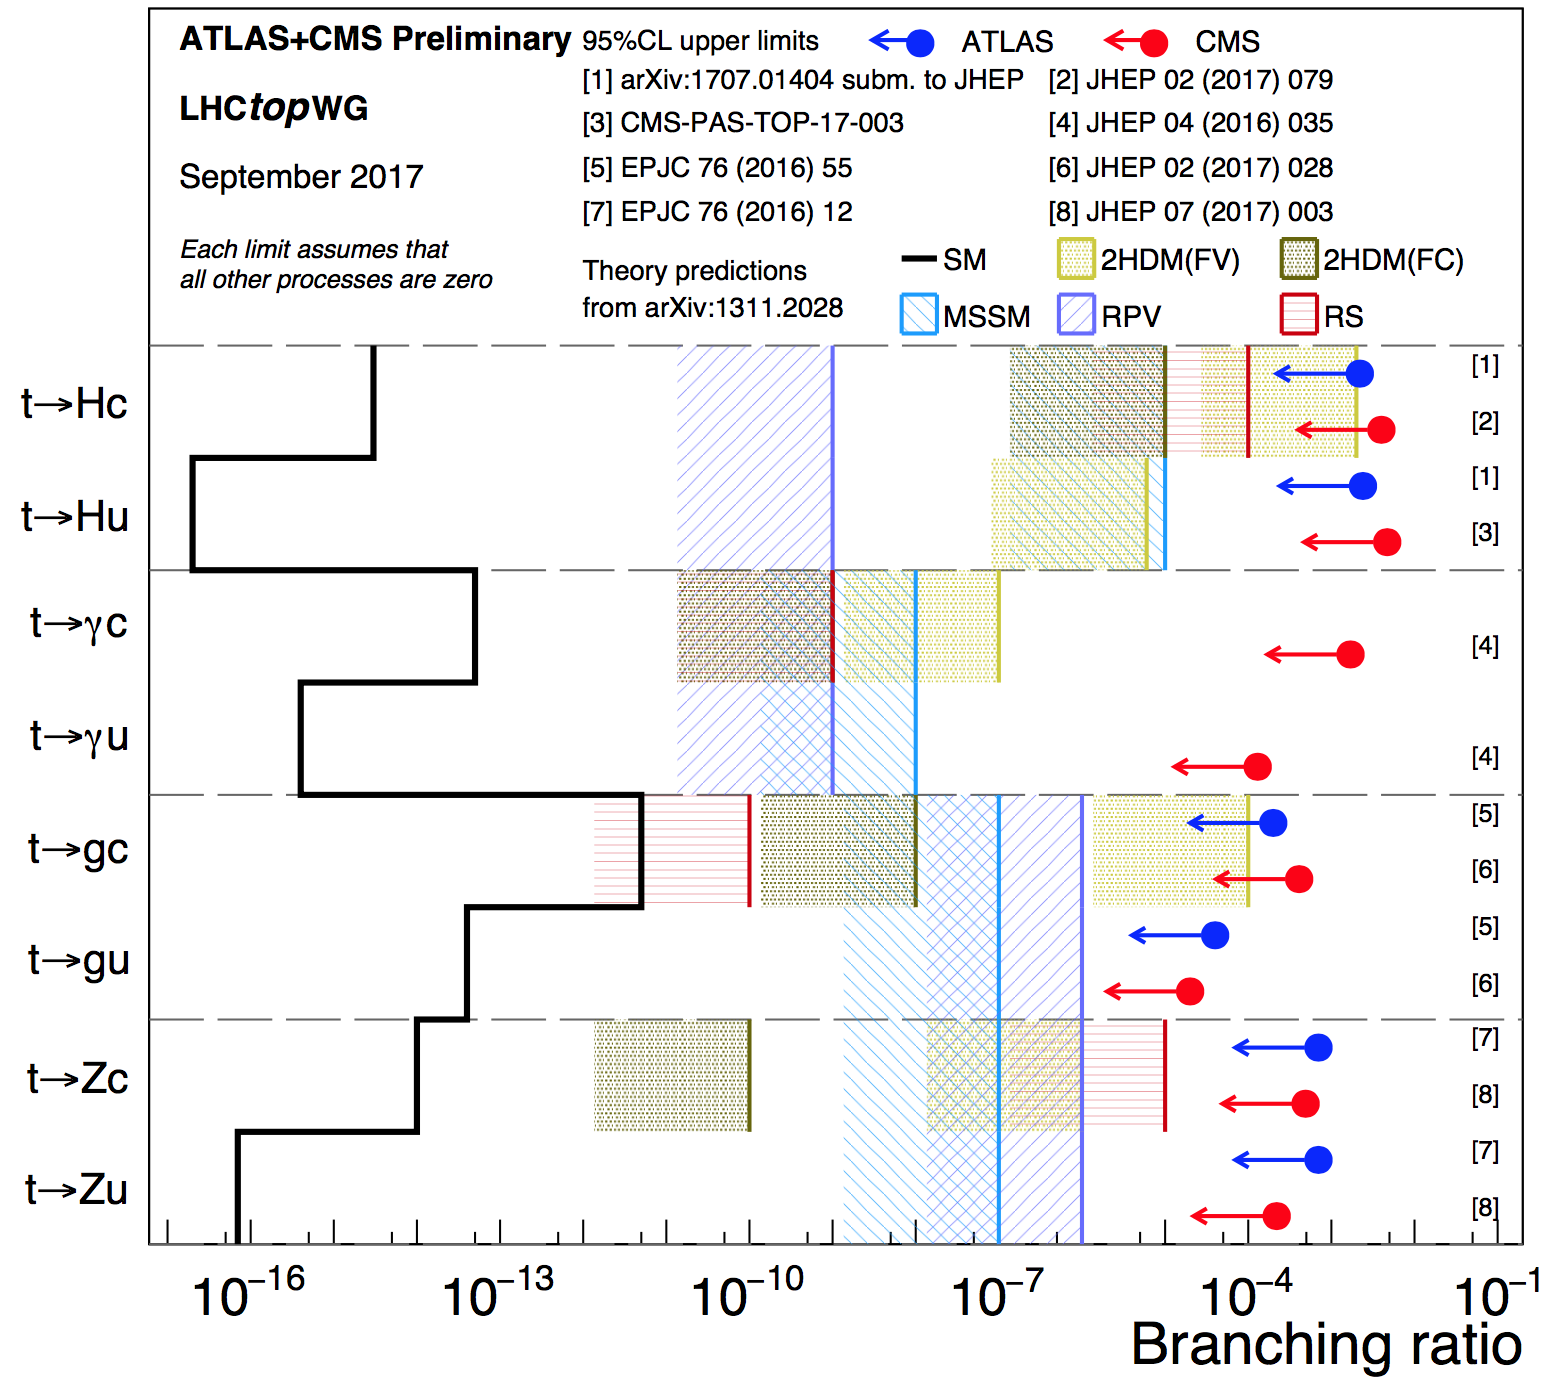
\includegraphics[width=0.7\linewidth]{1_Introduction/Figures/fcnc_summarybsm_sep17}
	\caption{Current best limits set by CMS and ATLAS for top-FCNC interactions.}
	\label{fig:fcncupperlimits}
\end{figure}



